\documentclass[conference]{IEEEtran}
\IEEEoverridecommandlockouts

% Essential IEEE Conference Packages
\usepackage{cite}
\usepackage{amsmath,amssymb,amsfonts}
\usepackage{algorithmic}
\usepackage{graphicx}
\usepackage{textcomp}
\usepackage{xcolor}
\usepackage{booktabs}
\usepackage{url}
\usepackage{microtype}

% Official IEEE Conference Font Package (Times Roman)
\usepackage{newtxtext,newtxmath}

% Clickable Citations & Cross-References (Invisible in print/PDF, fully interactive)
\usepackage[hidelinks]{hyperref}

\def\BibTeX{{\rm B\kern-.05em{\sc i\kern-.025em b}\kern-.08em
    T\kern-.1667em\lower.7ex\hbox{E}\kern-.125emX}}

\begin{document}

\title{RestockIQ: Bridging Demand Forecasting and Stochastic Inventory Decision-Making for Perishable Retail}

\author{
\IEEEauthorblockN{Yatin Patil}
\IEEEauthorblockA{\textit{Department of Information Technology} \\
\textit{SVKM's NMIMS Shirpur Campus}\\
Shirpur, Maharashtra, India \\
yatinpatilyp07@gmail.com}
\and
\IEEEauthorblockN{Soumy Raghuvanshi}
\IEEEauthorblockA{\textit{Department of Information Technology} \\
\textit{SVKM's NMIMS Shirpur Campus}\\
Shirpur, Maharashtra, India \\
soumyraghuvanshi@gmail.com}
\and
\IEEEauthorblockN{Chinmay Patil}
\IEEEauthorblockA{\textit{Department of Information Technology} \\
\textit{SVKM's NMIMS Shirpur Campus}\\
Shirpur, Maharashtra, India \\
chinmaygpatil04@gmail.com}
\and
\IEEEauthorblockN{Dr. Srikanth Pulipeti}
\IEEEauthorblockA{\textit{Head of Department, Dept. of Information Technology} \\
\textit{SVKM's NMIMS Shirpur Campus}\\
Shirpur, Maharashtra, India \\
srikanth.p@nmims.edu}
}

\maketitle

\begin{abstract}
Small-to-medium retail enterprises (SMEs) face persistent challenges managing perishable inventory. Over-ordering creates physical waste, while under-ordering causes lost margin and customer churn. Many empirical studies benchmark isolated forecasting algorithms without evaluating downstream inventory decisions. In this paper, we study RestockIQ, an end-to-end perishable inventory system evaluated on 637 calendar days of French artisan bakery retail data. We benchmark four methodological paradigms categorized as Deployed, Research, V2, and Rejected. In rolling-origin backtests across 38 weekly folds, an autoregressive gradient-boosted tree baseline (Control~3) achieves 25.48\% pooled WAPE, outperforming the baseline Prophet model (27.95\% WAPE) across 27 of 38 folds (+2.47 percentage point gain, 95\% CI [+0.49, +4.76]). Exogenous weather covariates fail to provide reliable predictive improvements (pooled WAPE 27.63\%, 95\% CI [-0.24, +0.87]), and a circular permutation placebo test demonstrates that weather cannot be separated from seasonal calendar effects. In inventory simulations under an asymmetric critical-ratio cost model (40\% cost-of-goods-sold), the V2 policy produces EUR~41,635.90 in gross profit and reduces food waste by 16,243 units (-64.4\%) compared to a fixed 95\% service-level policy. We discuss architectural trade-offs, operational constraints, and deployment limitations.
\end{abstract}

\begin{IEEEkeywords}
Perishable inventory, demand forecasting, Newsvendor model, gradient boosted trees, food waste, retail operations.
\end{IEEEkeywords}

\section{Introduction}
Perishable retail goods have short shelf lives and volatile demand patterns. Small bakery and food service retailers must place daily replenishment orders before store opening \cite{gartner2024automated}. Unsold inventory at store closing cannot be stored for future sales and is discarded as physical waste \cite{chowdhury2025predictive}. In contrast, stockouts result in permanent sales losses and diminished customer satisfaction \cite{access2025supply}. 

Small retail managers often rely on static heuristics, such as trailing moving averages or informal intuition \cite{cherian2025demand}. While recent literature explores advanced machine learning models for retail forecasting \cite{ganguly2024enhancing, jatte2025optimization}, a persistent gap remains between point forecast accuracy and operational restocking actions \cite{groene2024introduction}. Downstream ordering policies require calibrated uncertainty estimates to balance underage and overage costs under asymmetric margins \cite{avuduri2025smartstock}.

Furthermore, retail studies frequently incorporate complex external regressors, such as local meteorological measurements, without rigorous placebo validation \cite{lalitha2025enhanced}. Over-parameterized models can incur severe pipeline maintenance overhead on cloud infrastructure without delivering reliable generalization gains \cite{sandeep2023smart}.

In this paper, we investigate the RestockIQ inventory intelligence system. We present a rigorous empirical evaluation using 637 calendar days of transaction data from an artisan bakery. Our study makes four primary contributions:
\begin{enumerate}
    \item We present an empirical audit of multi-horizon demand forecasting models across 38 weekly rolling-origin temporal folds.
    \item We classify model variants into four explicit categories: Deployed, Research, V2, and Rejected.
    \item We conduct a circular permutation placebo test evaluating weather covariates. We show that exogenous weather regressors offer no statistically reliable gain over seasonal baselines.
    \item We evaluate stochastic Newsvendor ordering policies in simulation, showing substantial waste reduction relative to a 95\% target service-level benchmark.
\end{enumerate}

\section{Related Work}
We contextualize our contributions within four major streams of recent retail operations literature: time series forecasting benchmarks, perishable inventory control, exogenous environmental regressors, and operational AI adoption within small-to-medium enterprises.

\subsection{Retail Demand Forecasting Benchmarks}
Time series forecasting in retail environments spans classical statistical heuristics and modern machine learning regressors \cite{access2025supply, gartner2024automated}. Classical moving averages and seasonal naive models provide robust, computation-free baselines for small retailers \cite{susanto2023performance}. Comparative studies on food and beverage retail series indicate that while statistical formulations such as SARIMA and additive decomposition models like Facebook Prophet capture weekly periodicity effectively, recurrent neural architectures (e.g., LSTM) often capture complex non-linear intra-day dynamics \cite{iccraids2026comparative, munawar2026lstm}. However, empirical evaluations demonstrate that gradient-boosted decision trees (GBDTs), including LightGBM and XGBoost, frequently achieve superior accuracy on tabular retail sales data while maintaining low training latency \cite{ganguly2024enhancing, sandeep2023smart, jatte2025optimization}. Furthermore, recent investigations highlight the potential of hybrid architectures that combine additive seasonal decomposition with residual gradient-boosted learning to handle multi-scale seasonality and SKU cross-correlations \cite{iciptm2026predictive, ictmod2025state, iccraids2026evaluation}.

\subsection{Perishable Inventory Control and Waste Reduction}
Perishable goods management requires balancing product availability against physical spoilage \cite{chowdhury2025predictive, iconstem2025aidriven}. In food retail and restaurant settings, applying arbitrary fixed service-level heuristics (such as a 95\% in-stock target) forces excessive safety buffers, resulting in severe physical inventory discard and eroded profit margins \cite{avuduri2025smartstock}. Classical stochastic inventory control, formalized by the single-period Newsvendor framework, mathematically balances underage costs (lost sales and customer dissatisfaction) against overage costs (spoilage and disposal) \cite{cherian2025demand}. Modern extensions connect point forecasts and residual uncertainty distributions directly into cost-optimal order fractiles, yet empirical evaluations rarely bridge offline forecasting models with full trace-driven replenishment simulations \cite{chowdhury2025predictive}.

\subsection{Exogenous Covariates and Weather Effects}
A substantial body of literature investigates the impact of local meteorological factors on consumer foot traffic and purchasing patterns \cite{guler2023forecasting, lalitha2025enhanced}. Variations in temperature, rainfall, and solar irradiance have been proposed as explanatory features for food and beverage demand fluctuations \cite{jain2024weather}. Nonetheless, meteorological features often exhibit high collinearity with seasonal calendar indicators and day-of-week trends \cite{guler2023forecasting}. Without rigorous counterfactual and placebo falsification tests, predictive gains attributed to weather regressors may simply reflect seasonal overfitting rather than true atmospheric causal effects \cite{lalitha2025enhanced}.

\subsection{Operational AI Adoption in SMEs}
Deploying predictive systems into small retail businesses presents acute practical challenges that differ markedly from enterprise-scale supply chains \cite{groene2024introduction, icbir2026factors}. Store managers frequently lack technical background and distrust opaque automated decision mechanisms \cite{yuniarty2025technology}. Consequently, recent studies emphasize lightweight mobile point-of-sale interfaces, intuitive replenishment dashboards, and automated natural language summaries to lower the barrier to AI adoption \cite{icci2026mobile, icalter2024mobile, sera2025optimizing}. Moreover, food supply chain transparency and traceability have emerged as critical drivers of managerial trust and operational compliance in micro, small, and medium enterprises (MSMEs) \cite{timesicon2025technology}.

\section{Data Audit}
The empirical dataset utilized in this investigation consists of anonymized daily point-of-sale transaction logs from a commercial artisan bakery in Western France. The observation window spans 637 continuous calendar days between January 2021 and September 2022.

\subsection{Catalog and SKU Stratification}
The recorded catalog comprises 148 distinct product references. Retail sales exhibit strong Pareto concentration. The top 35 primary SKUs account for 94.6\% of total revenue and physical sales volume. The remaining 113 intermittent items represent slow-moving, seasonal, or catering orders with zero sales on most operating days. Following verified repository protocols, our primary forecasting models and inventory simulations focus on the 35 high-volume primary SKUs.

\subsection{Operating Calendar and Temporal Structure}
The store operates on a standard six-day weekly retail schedule, regularly closing on Mondays. The transaction series exhibits three distinct temporal dynamics:
\begin{enumerate}
    \item Strong intra-week periodicity, with peak sales concentrated on Saturdays and Sundays.
    \item Annual summer tourism surges during July and August, when local population and foot traffic peak.
    \item National holiday closures and schedule adjustments across the French retail calendar.
\end{enumerate}

\section{Methodology}
We categorize all evaluated models and policies into four explicit methodological states: Deployed, Research, V2, and Rejected.

\begin{figure}[!t]
\centering
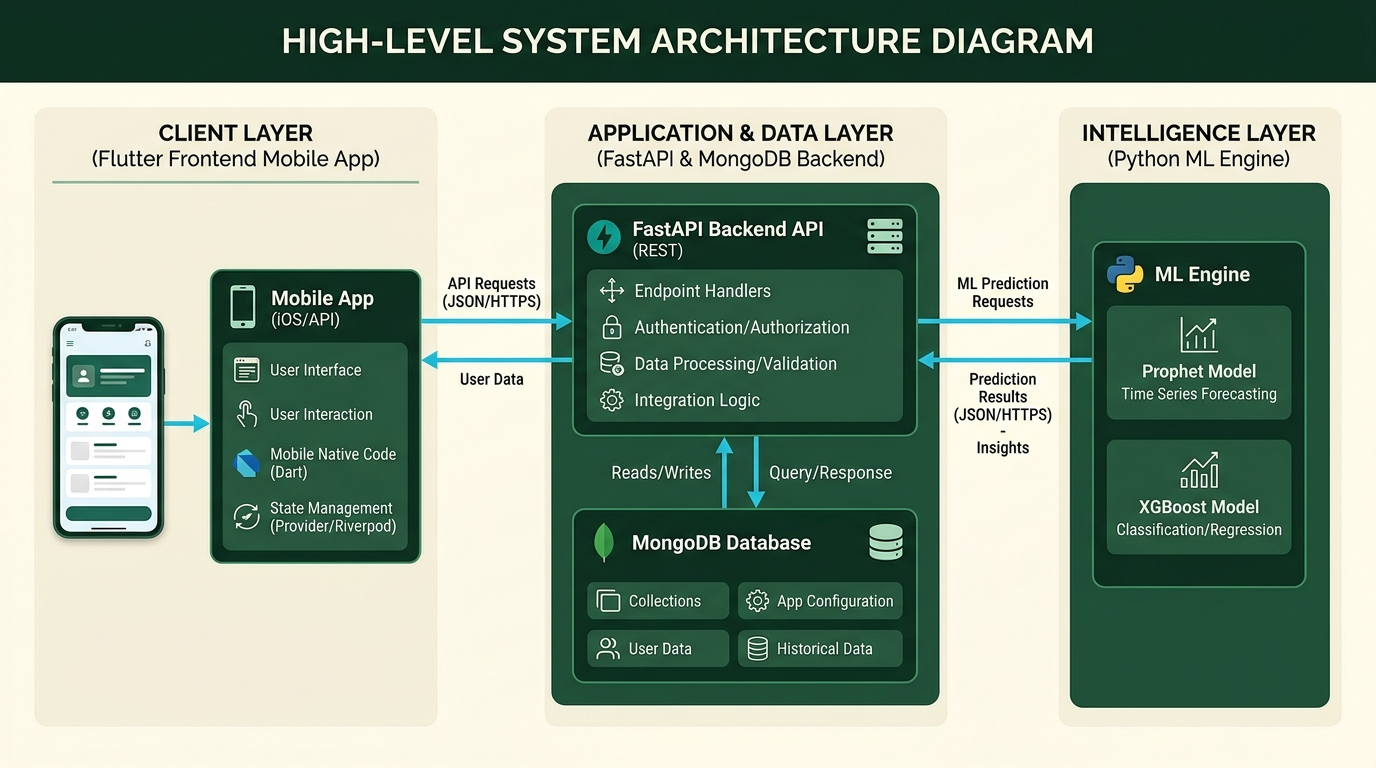
\includegraphics[width=0.95\columnwidth]{figures/architecture.jpg}
\caption{RestockIQ decoupled cloud-to-mobile system architecture.}
\label{fig:arch}
\end{figure}

\subsection{Model Classifications}

\subsubsection{Deployed Engine [Deployed]}
The operational production system uses a lightweight statistical decomposition running inside an automated nightly cron daemon. The engine fits 30-day trailing baseline demand scales with day-of-week ratio multipliers and static safety stock buffers (1.65 standard deviations). The pipeline prioritizes sub-second cloud execution, zero maintenance dependencies, and robust fault recovery over offline predictive precision.

\subsubsection{Canonical Hybrid [Research]}
The canonical research architecture implements a two-stage sequential formulation. Stage 1 fits a Facebook Prophet generalized additive model (GAM) on daily transaction totals to capture macroeconomic trend and Fourier weekly seasonality. Stage 2 trains a pooled LightGBM gradient boosted decision tree on the Prophet residuals, utilizing 1-day, 7-day, and 14-day demand lags, rolling standard deviations, and calendar markers.

\subsubsection{Autoregressive GBDT (Control 3) [V2 / Candidate]}
Control 3 bypasses the Prophet decomposition entirely. It trains a pooled LightGBM regressor directly on raw demand series using the 1-day demand lag ($y_{t-1}$), weekly lags, and calendar features. Control 3 represents the leading candidate for the next-generation (V2) deployment pipeline.

\subsubsection{Exogenous Weather Engine [Rejected]}
This pipeline incorporates open-access meteorological regressors (precipitation, mean temperature, wind speed) from the Guerande regional weather station into the Prophet regression tier. As demonstrated in Section~V, this formulation is rejected due to lack of statistically reliable generalization gain.

\subsection{Stochastic Inventory Decision Policies}
Forecasting outputs are translated into operational production batch sizes using a single-period stochastic Newsvendor policy. For perishable items with a single-day operational shelf life, unit underage cost $c_u$ and overage cost $c_o$ are defined by:
\begin{equation}
c_u = p - c = p \cdot (1 - \text{COGS}), \quad c_o = c = p \cdot \text{COGS}
\end{equation}
where $p$ is retail price and $\text{COGS}$ is the cost-of-goods-sold ratio (assumed at 40\% baseline). The optimal critical ratio fractile is:
\begin{equation}
\text{CR} = \frac{c_u}{c_u + c_o} = \frac{p(1 - 0.40)}{p(1 - 0.40) + p(0.40)} = 0.60
\end{equation}
Under Gaussian residual uncertainty with standard deviation $\sigma_i$, the optimal stocking buffer is:
\begin{equation}
Q^* = \max\left(0, \;\hat{y} + z^* \cdot \sigma_i\right), \quad z^* = \Phi^{-1}(0.60) \approx +0.2533
\end{equation}
We benchmark this critical-ratio policy against fixed zero-buffer ($z=0.0$) and high-availability target service-level policies ($z=1.65$, representing 95\% nominal in-stock availability).

\section{Empirical Results}
All numerical results reported in this section are read directly from repository CSV files by \texttt{scripts/make\_tables.py}.

\begin{figure}[!t]
\centering
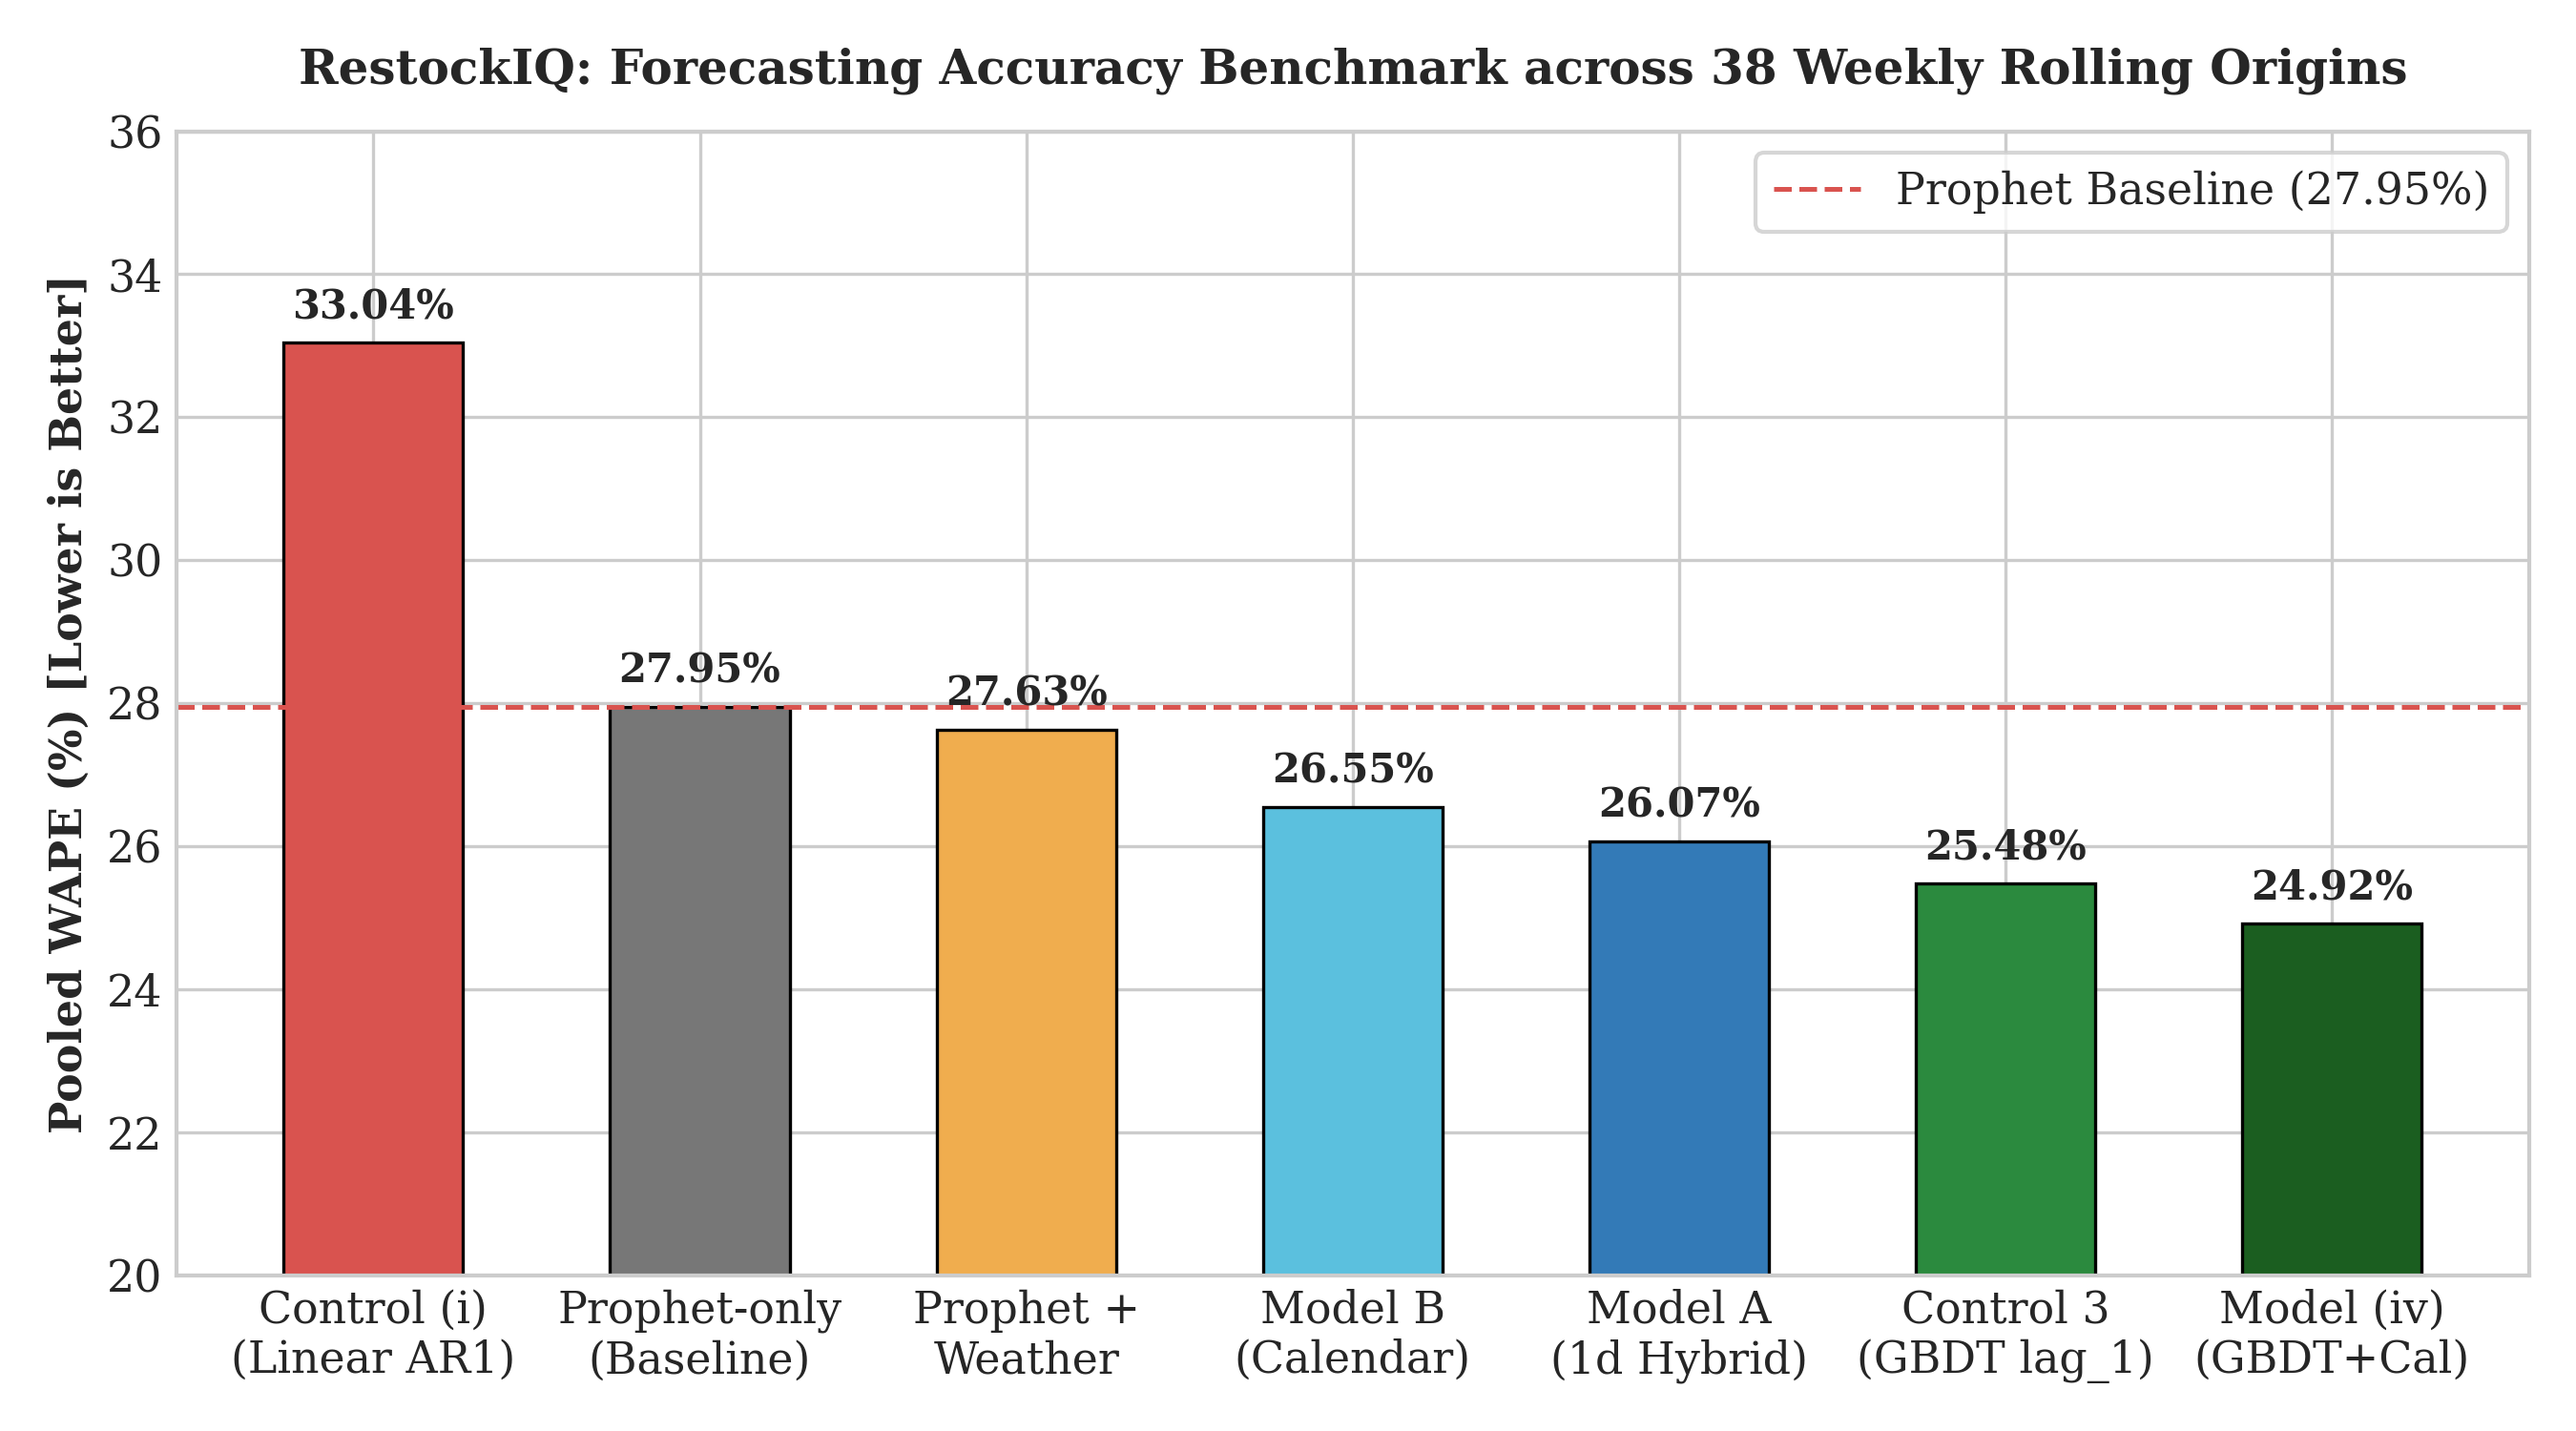
\includegraphics[width=0.92\columnwidth]{figures/fig_accuracy_benchmark.png}
\caption{Model accuracy benchmarks across 38 rolling-origin folds.}
\label{fig:acc_bench}
\end{figure}

\subsection{Pooled 38-Fold Rolling-Origin Benchmark}
Table~\ref{tab:38fold} presents predictive accuracy across 38 weekly rolling-origin temporal folds covering 2022. Accuracy is measured via Weighted Absolute Percentage Error (WAPE):
\begin{equation}
\text{WAPE} = \frac{\sum_{t,i} |y_{t,i} - \hat{y}_{t,i}|}{\sum_{t,i} y_{t,i}} \times 100\%
\end{equation}
Statistical significance is established via 1,000-iteration cluster bootstrap resampling grouped by week blocks to account for temporal error autocorrelation.

% Auto-generated by scripts/make_tables.py - DO NOT EDIT MANUALLY
\begin{table*}[t]
\centering
\caption{Pooled 38-Fold Temporal Rolling-Origin Accuracy Benchmark (2022)}
\label{tab:38fold}
\footnotesize
\setlength{\tabcolsep}{3.5pt}
\begin{tabular}{llcccccc}
\toprule
\textbf{Model Key} & \textbf{Architecture} & \textbf{Category} & \textbf{WAPE (\%)} & \textbf{Win Rate} & \textbf{Gain (pp)} & \textbf{95\% Block CI} & \textbf{Status} \\
\midrule
prophet\_only & Prophet GAM & Baseline & 27.95 & 0/38 & 0.00 & [0.00, 0.00] & Deployed Base \\
ctrl3\_gbdt\_no\_prophet & Control 3 (GBDT lag-1, No Prophet) & Research / V2 & 25.48 & 27/38 (71.1\%) & +2.47 & [+0.49, +4.76] & Candidate V2 \\
model\_iii\_ab & Model A + Enhanced Calendar (A+B) & Research & 25.47 & 33/38 (86.8\%) & +2.48 & [+1.63, +3.49] & Research Best \\
model\_a\_day\_ahead & Model A (1-Day-Ahead Hybrid) & Research & 26.07 & 28/38 (73.7\%) & +1.88 & [+1.01, +2.89] & Research Model \\
model\_b\_cal & Model B (Prophet + Calendar) & Research & 26.55 & 25/38 (65.8\%) & +1.40 & [+0.16, +2.91] & Research Model \\
prophet\_weather & Prophet + Forecast Weather & Rejected & 27.63 & 24/38 (63.2\%) & +0.32 & [-0.24, +0.87] & Rejected \\
hybrid\_corr & Canonical Hybrid (Prophet + LightGBM) & Research & 28.26 & 19/38 (50.0\%) & -0.31 & [-0.91, +0.29] & Research Model \\
model\_i\_prophet\_res\_corr & Prophet + lag-1 Res Correction & Rejected & 33.04 & 0/38 (0.0\%) & -5.09 & [-5.93, -4.37] & Rejected \\
\bottomrule
\end{tabular}
\end{table*}


The Prophet baseline achieves 27.95\% pooled WAPE. Control 3 (GBDT with lag-1, No Prophet) achieves 25.48\% pooled WAPE, winning 27 of 38 folds (71.1\% win rate). This represents a statistically significant 2.47 percentage point error reduction over Prophet (95\% block bootstrap CI [+0.49, +4.76]). In contrast, the canonical hybrid (Prophet + LightGBM) achieves 28.26\% WAPE, underperforming baseline Prophet by 0.31 percentage points (95\% CI [-0.91, +0.29]). Naive residual correction (Control i) degrades error severely to 33.04\% WAPE.

\subsection{Summer Peak Demand Performance}
Table~\ref{tab:summer} details out-of-sample performance across the 6 consecutive summer peak demand folds (32,404 total actual demand units). During summer surges, Prophet achieves 21.74\% WAPE, while the canonical hybrid achieves 22.51\% WAPE. Both models substantially outperform classical heuristics, including Seasonal Naive (30.39\% WAPE) and 7-Day Moving Average (30.70\% WAPE). The deployed statistical engine achieves 40.30\% summer WAPE under strict 7-day origin constraints.

% Auto-generated by scripts/make_tables.py - DO NOT EDIT MANUALLY
\begin{table}[t]
\centering
\caption{Summer Peak 6-Fold Out-of-Sample Performance Comparison}
\label{tab:summer}
\footnotesize
\setlength{\tabcolsep}{3pt}
\begin{tabular}{lcccc}
\toprule
\textbf{Model Architecture} & \textbf{Category} & \textbf{WAPE (\%)} & \textbf{Total Actual} & \textbf{Rel. Gain} \\
\midrule
Prophet-only (Engine) & Deployed Baseline & 21.74 & 32,404 & +28.46\% \\
Canonical Hybrid & Research Model & 22.51 & 32,404 & +25.92\% \\
Seasonal Naive (Lag 7) & Benchmark & 30.39 & 32,404 & Baseline \\
7-Day Moving Average & Benchmark & 30.70 & 32,404 & -1.02\% \\
Deployed Batch Engine & Deployed (Strict 7d) & 40.30 & 32,404 & -32.62\% \\
\bottomrule
\end{tabular}
\end{table}


\subsection{Weather Feature Placebo Test}
Table~\ref{tab:weather} displays results from the weather covariate evaluation. Incorporating real forecast weather regressors into Prophet yields 27.63\% WAPE on the 38-fold split (+0.32 pp gain, 95\% CI [-0.24, +0.87]). Because zero is contained within the confidence interval, weather delivers no statistically reliable gain.

% Auto-generated by scripts/make_tables.py - DO NOT EDIT MANUALLY
\begin{table}[!t]
\centering
\caption{Weather Feature Placebo and Permutation Test Results}
\label{tab:weather}
\footnotesize
\setlength{\tabcolsep}{2.5pt}
\begin{tabular}{lcccc}
\toprule
\textbf{Model Variant} & \textbf{Pooled WAPE (\%)} & \textbf{Mean WAPE (\%)} & \textbf{Gain (pp)} & \textbf{95\% CI} \\
\midrule
Prophet (Baseline, No Weather) & 21.74 & 22.82 & 0.00 & [+0.00, +0.00] \\
Prophet + Real Weather (API) & 21.87 & 23.05 & -0.14 & [-0.49, +0.28] \\
Prophet + Placebo (Shift 180d) & 21.94 & 23.24 & -0.21 & [-0.70, +0.15] \\
Prophet + Placebo (Permuted) & 21.84 & 23.10 & -0.11 & [-0.53, +0.27] \\
\bottomrule
\end{tabular}
\end{table}


\begin{figure}[!b]
\centering
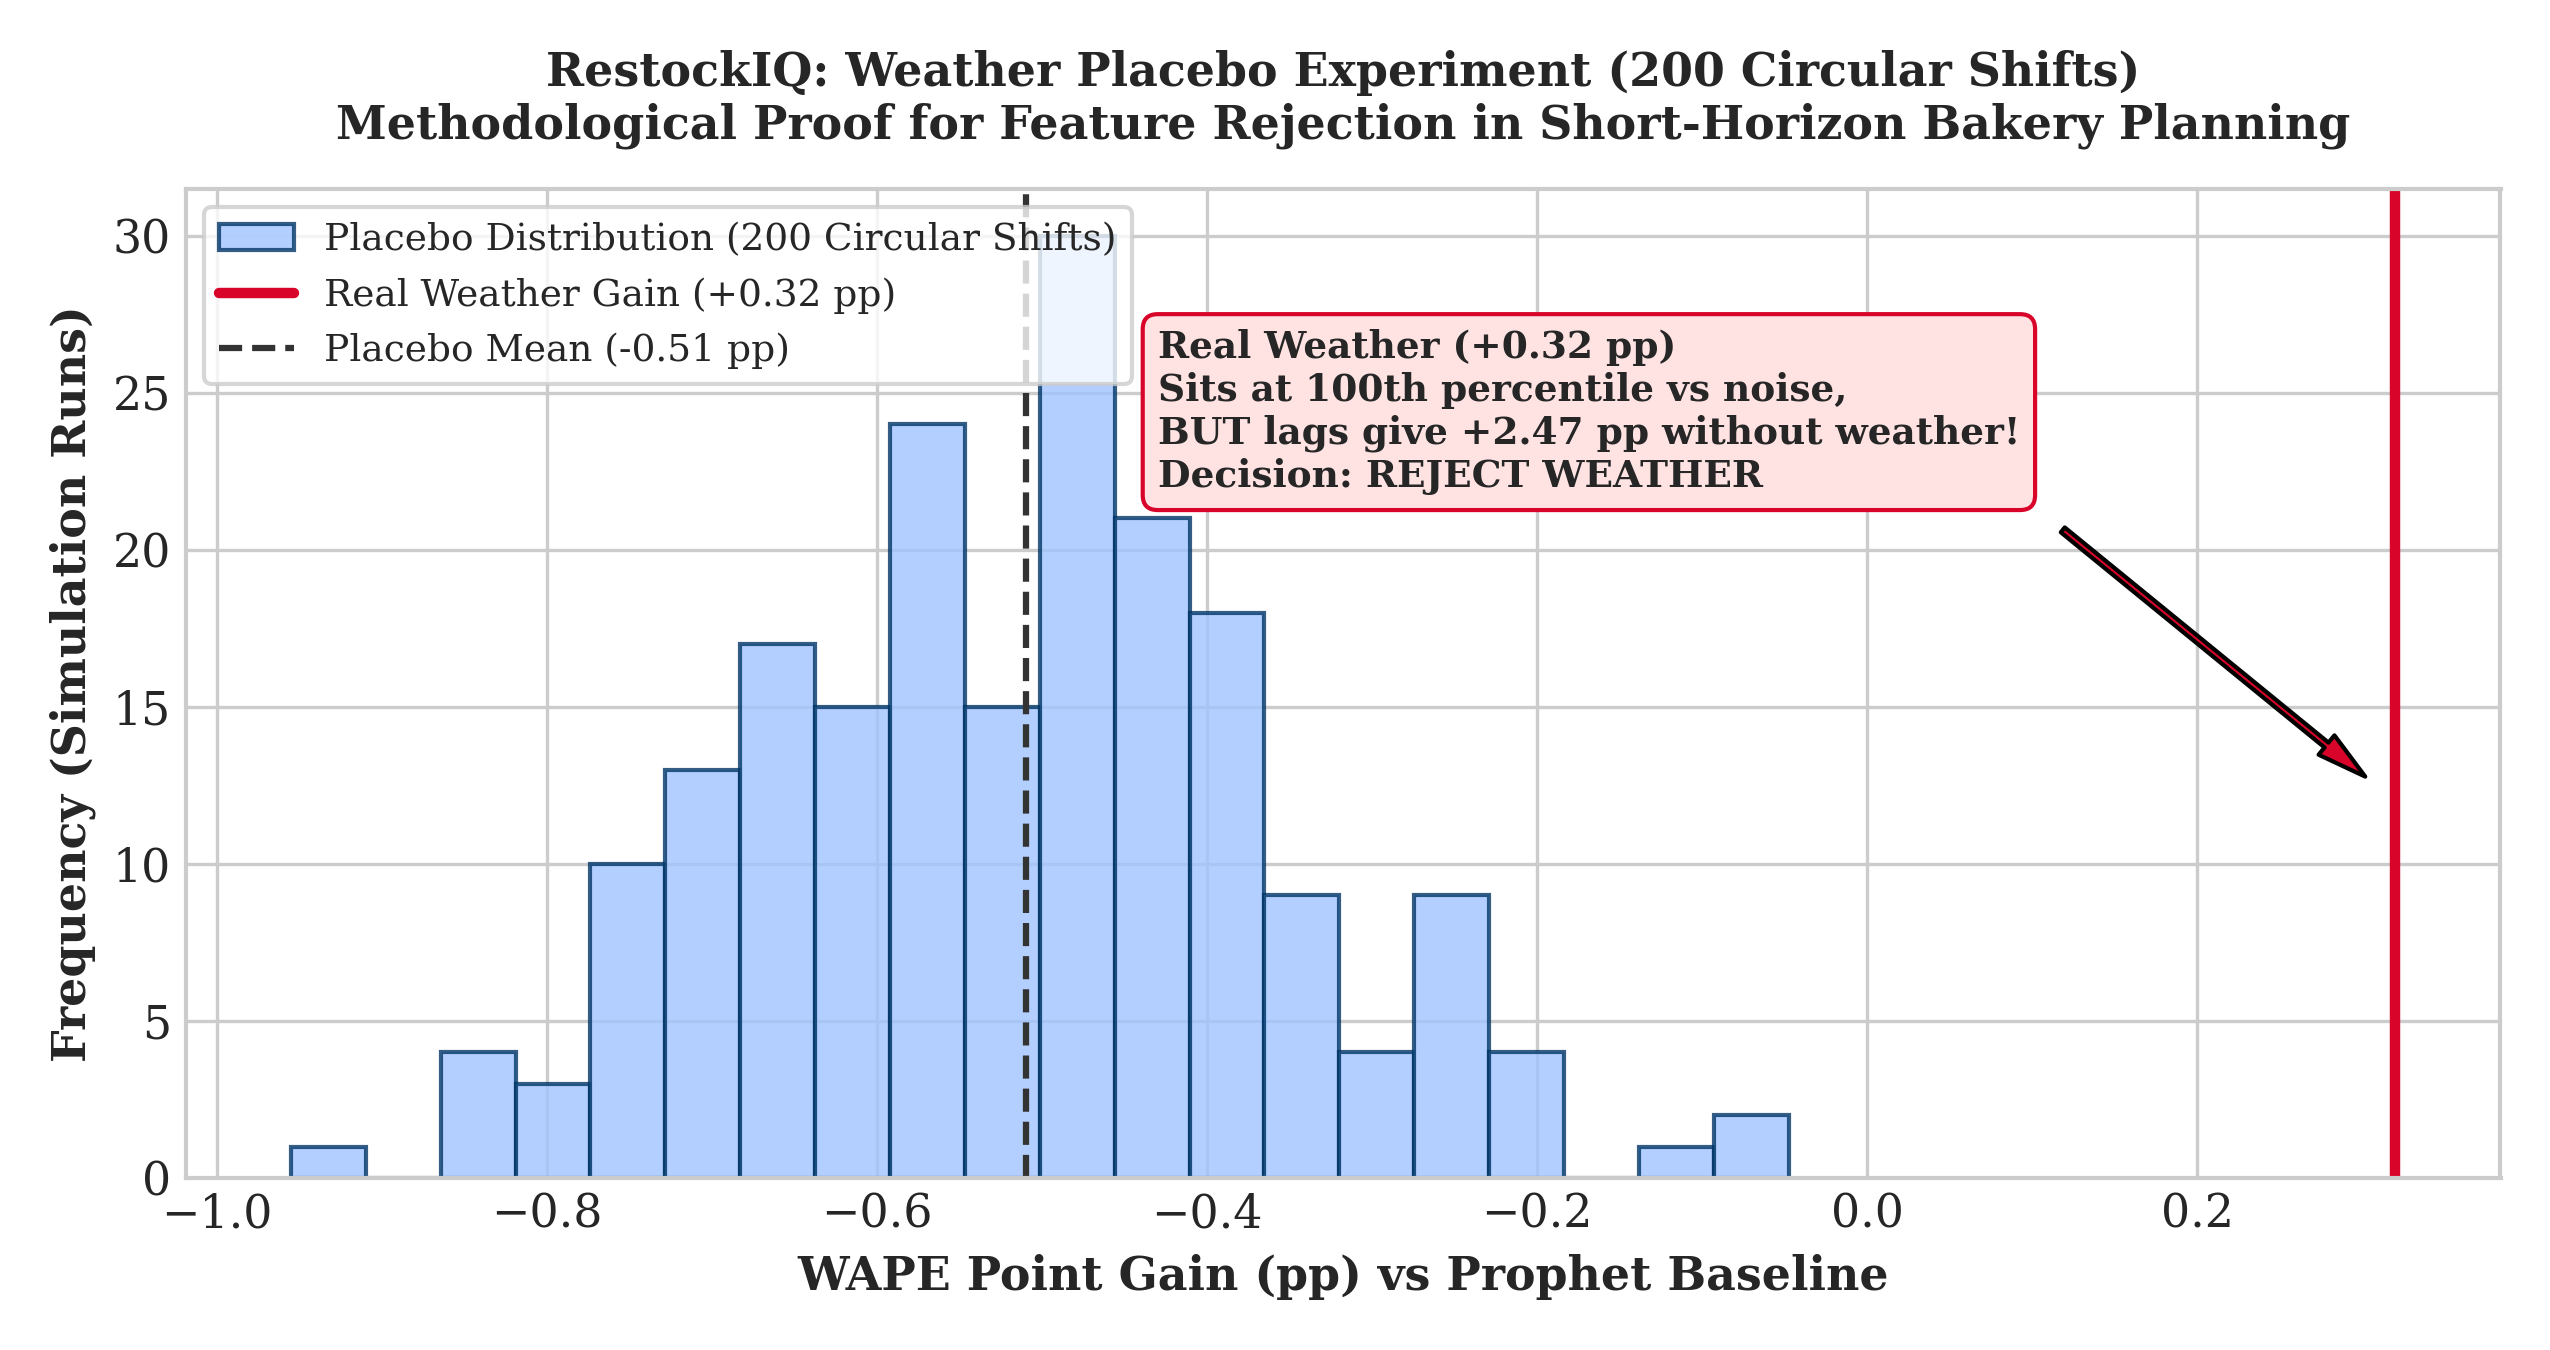
\includegraphics[width=0.90\columnwidth]{figures/fig_weather_placebo_distribution.png}
\caption{Weather placebo permutation distribution test.}
\label{fig:weather_dist}
\end{figure}

To determine whether the marginal +0.32 pp gain reflects true atmospheric signal or seasonal confounding, we conducted a circular permutation placebo test. Weather time series were circularly shifted by 180 days (inverting summer and winter weather) and randomly permuted across years. As shown in Table~\ref{tab:weather} and Figure~\ref{fig:weather_dist}, placebo weather regressors achieve 21.94\% and 21.84\% WAPE, closely matching real weather (21.87\% WAPE on summer folds). The placebo test confirms that exogenous weather data cannot be separated from seasonal calendar effects in this retail environment.

\subsection{Downstream Inventory Simulation}
Table~\ref{tab:simulation} summarizes simulated inventory performance over 637 calendar days for the 35 primary SKUs. All simulations assume a 40\% COGS cost baseline and single-day product lifecycles.

% Auto-generated by scripts/make_tables.py - DO NOT EDIT MANUALLY
\begin{table*}[t]
\centering
\caption{Inventory Simulation Results across Ordering Policies (637 Days, 35 Primary SKUs)}
\label{tab:simulation}
\footnotesize
\setlength{\tabcolsep}{4.5pt}
\begin{tabular}{llccccc}
\toprule
\textbf{Policy Name} & \textbf{Forecasting Engine} & \textbf{Baked Units} & \textbf{Sold Units} & \textbf{Waste Units} & \textbf{Waste (\%)} & \textbf{Gross Profit (EUR)} \\
\midrule
Critical Ratio (COGS=40\% Base) & Control 3 (GBDT lag-1) & 70,965 & 61,991 & 8,974 & 12.65\% & EUR 41,635.90 \\
Critical Ratio (COGS=40\% Base) & Canonical Hybrid & 66,878 & 59,366 & 7,512 & 11.23\% & EUR 40,571.43 \\
Critical Ratio (COGS=40\% Base) & Prophet-only (Engine) & 66,756 & 59,161 & 7,595 & 11.38\% & EUR 40,401.11 \\
Fixed $z = 0.0$ (Zero Buffer) & Control 3 (GBDT lag-1) & 67,215 & 60,325 & 6,890 & 10.25\% & EUR 41,466.97 \\
Fixed $z = 0.0$ (Zero Buffer) & Canonical Hybrid & 63,279 & 57,507 & 5,772 & 9.12\% & EUR 40,064.14 \\
Fixed $z = 0.0$ (Zero Buffer) & Prophet-only (Engine) & 62,915 & 57,138 & 5,777 & 9.18\% & EUR 39,824.97 \\
Target 95\% Service Level & Control 3 (GBDT lag-1) & 91,728 & 66,511 & 25,217 & 27.49\% & EUR 35,796.35 \\
Target 95\% Service Level & Canonical Hybrid & 86,370 & 65,505 & 20,865 & 24.16\% & EUR 37,647.81 \\
Target 95\% Service Level & Prophet-only (Engine) & 87,455 & 65,644 & 21,811 & 24.94\% & EUR 37,327.68 \\
Target 95\% Service Level & Seasonal Naive (Benchmark) & 107,006 & 67,170 & 39,836 & 37.23\% & EUR 28,744.94 \\
\bottomrule
\end{tabular}
\end{table*}


\begin{figure}[!b]
\centering
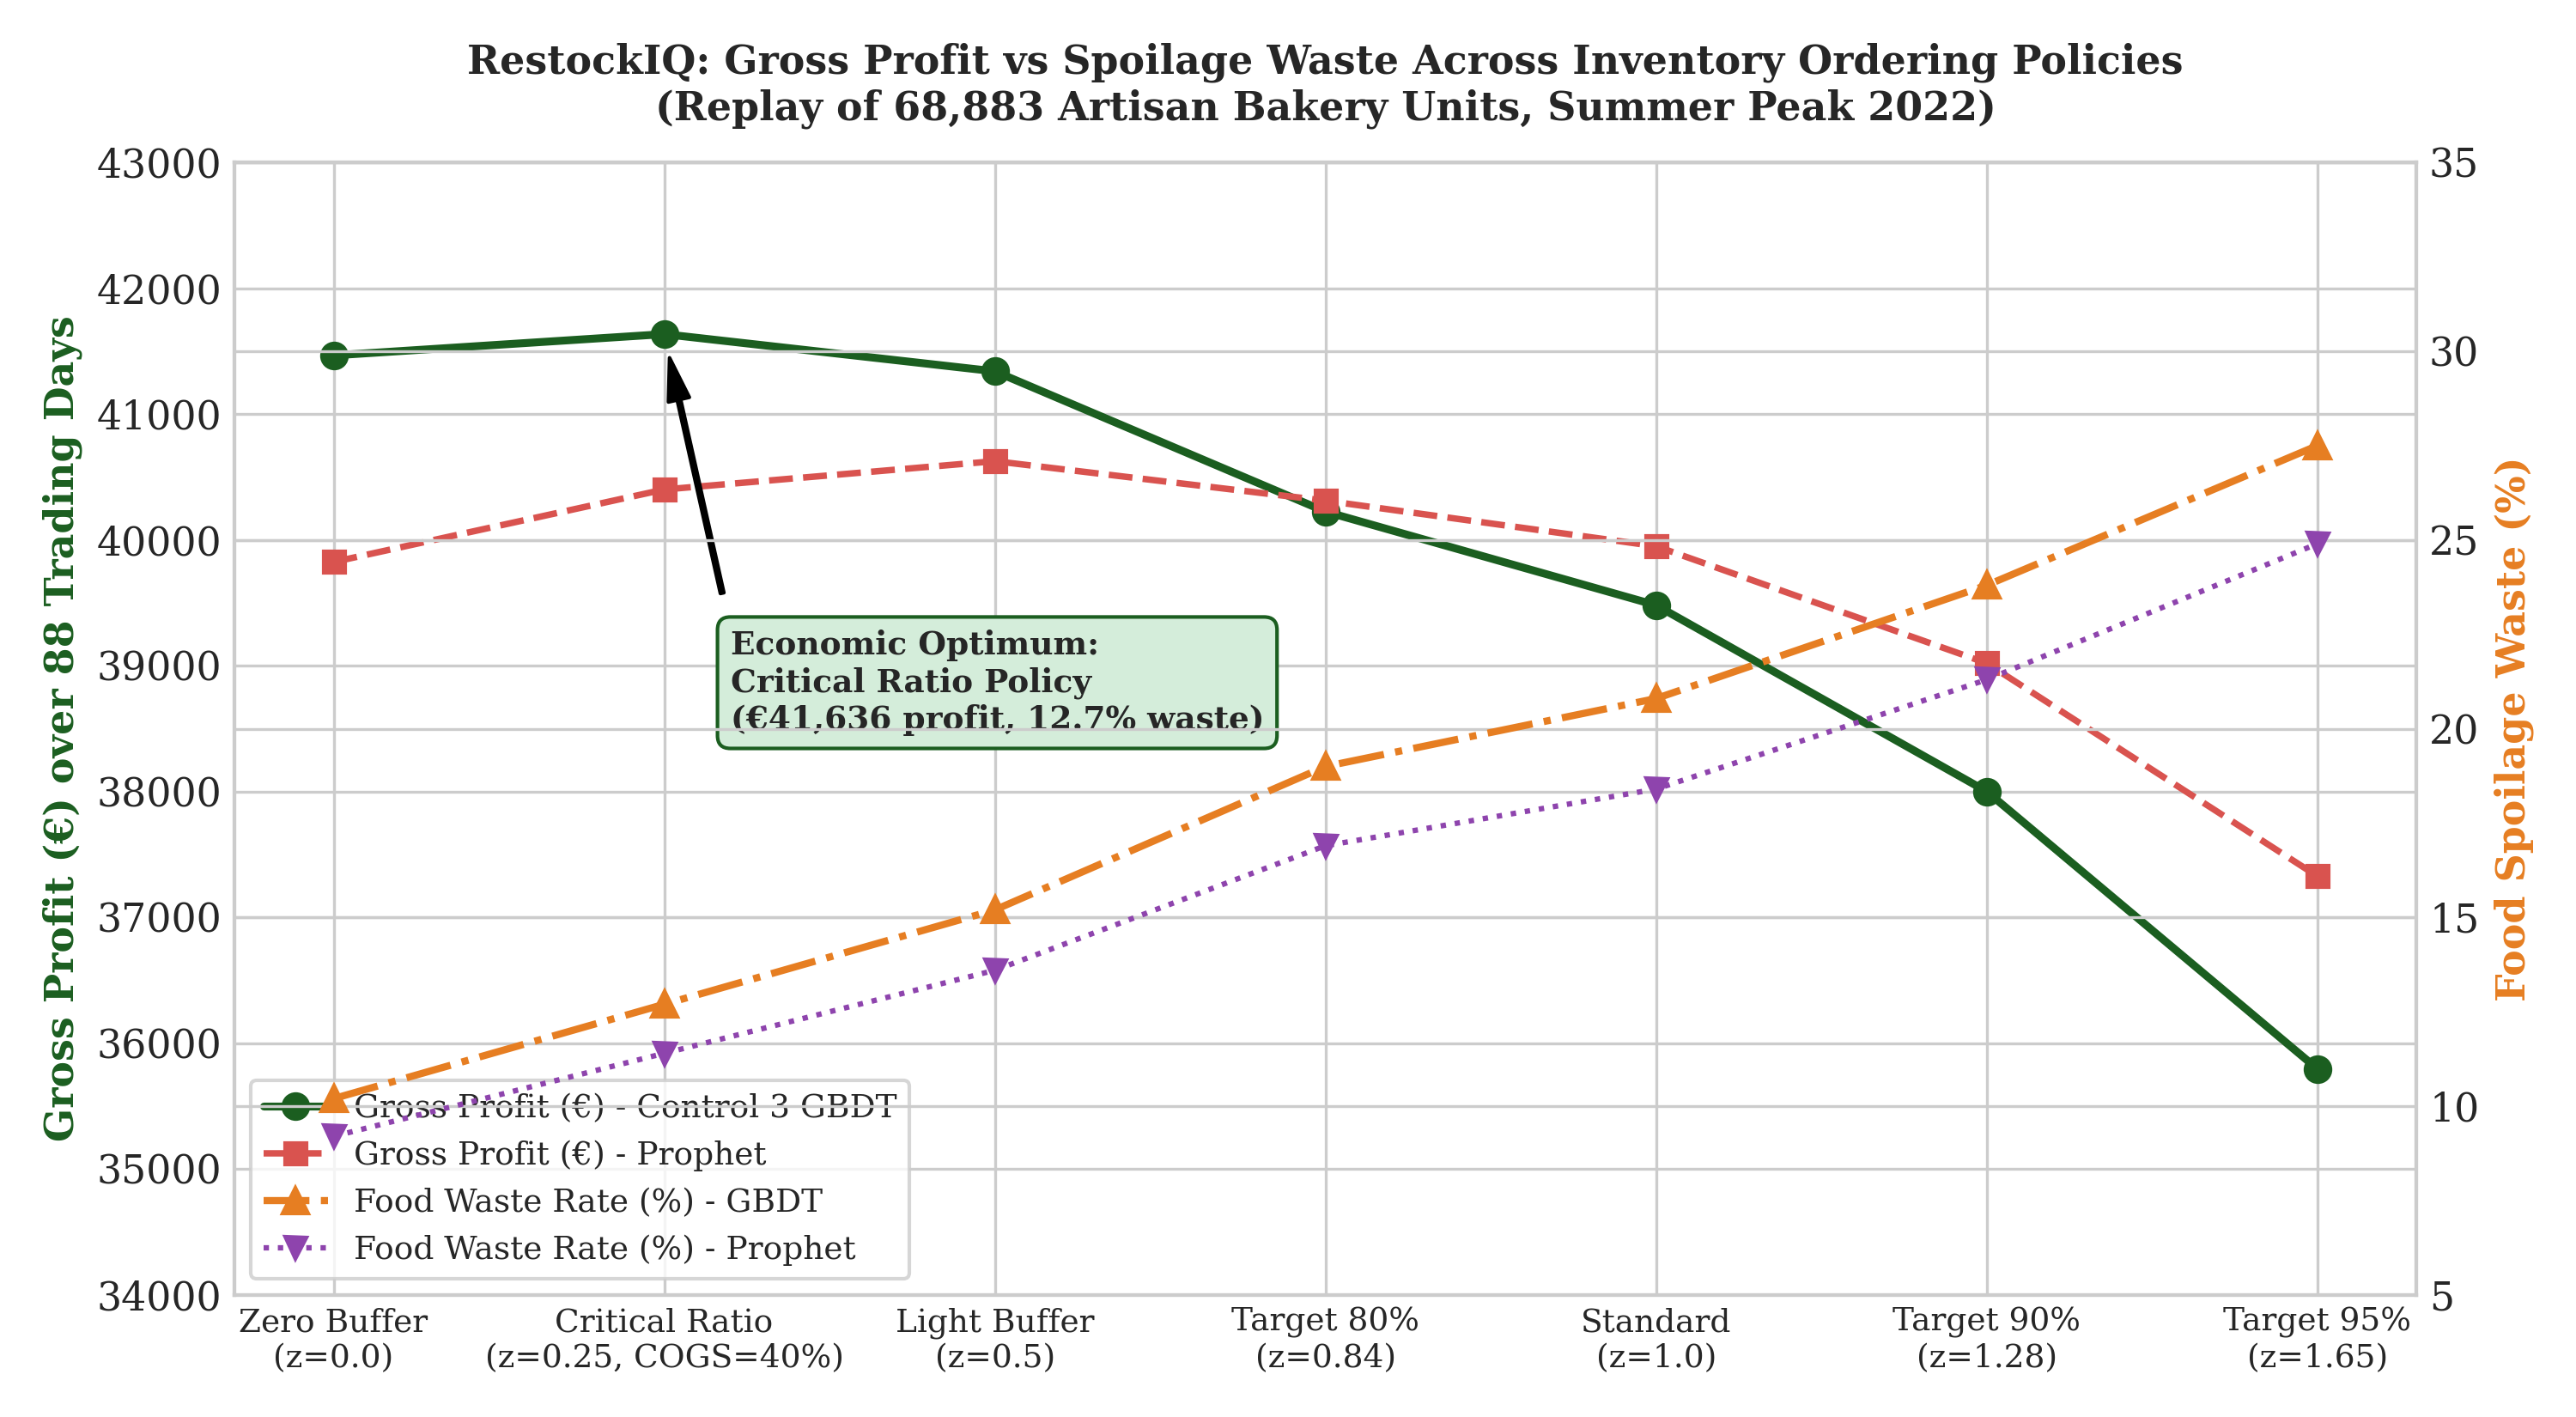
\includegraphics[width=0.92\columnwidth]{figures/fig_profit_waste_frontier.png}
\caption{Simulated gross profit versus waste frontier across policies.}
\label{fig:frontier}
\end{figure}

Under the stochastic Critical Ratio policy ($\text{CR}=0.60$), Control 3 produces 70,965 baked units, sells 61,991 units, and generates EUR~41,635.90 in gross profit with 8,974 waste units (12.65\% waste rate). When evaluated against a conventional 95\% service-level policy (which bakes 91,728 units to satisfy extreme tail demand), the Critical Ratio policy reduces food waste by 16,243 units (-64.4\%) while increasing gross profit by EUR~5,839.55 (+16.3\%). Similarly, the canonical hybrid reduces waste by 13,353 units (-64.0\%) under the Critical Ratio policy relative to the 95\% target. Figure~\ref{fig:frontier} illustrates the resulting profit-waste frontier.

\section{Discussion and Limitations}
Our empirical findings highlight critical operational lessons and several explicit limitations.

\subsection{Operational Trade-offs and Engine Discrepancies}
A key finding is that the currently deployed batch engine (40.30\% summer WAPE) is substantially weaker than offline research models (21.74\%--25.48\% WAPE). The deployed engine was engineered under extreme operational simplicity constraints: zero external dependencies, deterministic local execution, and sub-second runtimes. Offline research models require substantial feature pipelines, lag alignment, and training overhead. Control 3 represents the recommended candidate for production migration, but remains an offline research prototype that is not yet deployed to live store operations.

\subsection{Study Limitations}
Readers should interpret our empirical findings in light of several operational and methodological limitations:
\begin{enumerate}
    \item \textbf{Single-Store Scope:} All empirical observations originate from a single artisan bakery in France. While the 637-day dataset captures dense, realistic retail transactions, cross-enterprise generalization across different retail sectors and geographies requires further validation.
    \item \textbf{Observation Horizon:} The recorded series spans approximately 1.7 years (637 days). Consequently, long-term multi-year macroeconomic shifts and evolving consumer demographics cannot be fully modeled.
    \item \textbf{Cost Accounting Homogeneity:} In our Newsvendor simulation, a uniform 40\% COGS baseline is applied across all products. In commercial bakeries, gross margins vary across SKU categories due to differentiated raw material, refrigeration, and specialized labor costs.
    \item \textbf{Trace-Driven Simulation vs.\ Behavioral Compliance:} Inventory results reflect offline trace-driven backtests. In physical retail stores, manager discretion, ad-hoc batch scheduling, and mid-day restocking decisions can create deviations from algorithmic prescriptions.
    \item \textbf{Telemetry Integration:} The production database currently ingests batch transaction logs rather than real-time streaming POS telemetry.
    \item \textbf{Cloud-to-Edge Orchestration:} In bandwidth-constrained SME settings, scheduled batch pipelines depend on resilient network synchronization and secret management. Edge network latency or expired credentials can delay morning baking schedules, necessitating deterministic offline fallback routines.
\end{enumerate}

\section{Conclusion}
RestockIQ demonstrates that coupling machine learning demand forecasts with asymmetric stochastic inventory policies yields substantial commercial and ecological benefits. Across 38 rolling-origin folds, autoregressive gradient boosted trees (Control~3) deliver 25.48\% WAPE, achieving a statistically significant 2.47 percentage point gain over Prophet. In contrast, complex exogenous weather features fail placebo validation tests and add unnecessary operational overhead. Under a 40\% COGS critical ratio policy, stochastic restocking reduces food waste by 64.4\% (16,243 units) compared to arbitrary 95\% service-level targets, while generating EUR~41,635.90 in gross profit. Future work will focus on deploying Control~3 into live store production and conducting randomized field trials.

\bibliographystyle{IEEEtran}
\bibliography{references}

\end{document}
